%%%%%%%%%%%%%%%%%%%%%%%%%%%%%%%%%%%%%%%%%%%%%%%%%%%%%%%%%%%%%%%%%%%%%%%%%%%%%%%
% Neuroimage-like layout
\documentclass[5p]{elsarticle}
\usepackage{amsmath,amsfonts,amssymb}
\usepackage{bm}
\usepackage{algorithm}
\usepackage{algorithmic}
\usepackage{url}
\usepackage[breaklinks=true,letterpaper=true,colorlinks,bookmarks=false]{hyperref}
\usepackage[table]{xcolor}

\definecolor{deep_blue}{rgb}{0,.2,.5}
\definecolor{dark_blue}{rgb}{0,.15,.5}

\hypersetup{pdftex,  % needed for pdflatex
  breaklinks=true,  % so long urls are correctly broken across lines
  colorlinks=true,
  linkcolor=dark_blue,
  citecolor=deep_blue,
}

% Float parameters, for more full pages.
\renewcommand{\topfraction}{0.9}        % max fraction of floats at top
\renewcommand{\bottomfraction}{0.8}     % max fraction of floats at bottom
\renewcommand{\textfraction}{0.07}      % allow minimal text w. figs
%   Parameters for FLOAT pages (not text pages):
\renewcommand{\floatpagefraction}{0.6}  % require fuller float pages
%    % N.B.: floatpagefraction MUST be less than topfraction !!


\def\B#1{\mathbf{#1}}
%\def\B#1{\bm{#1}}
\def\trans{^\mathsf{T}}
% A compact fraction
\def\slantfrac#1#2{\kern.1em^{#1}\kern-.1em/\kern-.1em_{#2}}

%%%%%%%%%%%%%%%%%%%%%%%%%%%%%%%%%%%%%%%%%%%%%%%%%%%%%%%%%%%%%%%%%%%%%%%%%%%%%%%%
\begin{document}

%\title{Comparing Connectomes Between Populations}
\title{Learning and comparing functional connectomes between populations}


\author[parietal,unicog,cea]{Ga\"el Varoquaux\corref{corresponding}}
\author[cmi,nki]{R. Cameron Craddock}

\cortext[corresponding]{Corresponding author}

\address[parietal]{Parietal project-team, INRIA Saclay-\^ile de France}
\address[unicog]{INSERM, U992}
\address[cea]{CEA/Neurospin b\^at 145, 91191 Gif-Sur-Yvette}
\address[cmi]{Child Mind Institute, New York, New York}
\address[nki]{Nathan Kline Institute for Psychiatric Research, Orangeburg, New York}

\begin{abstract}
    We are the champion... of the world

    Scope: rest and task-based studies. But focusing on fMRI.
\end{abstract}

\begin{keyword}
    Functional connectivity, connectome, group study, effective
    connectivity, fMRI, resting-state
\end{keyword}

\maketitle
%%%%%%%%%%%%%%%%%%%%%%%%%%%%%%%%%%%%%%%%%%%%%%%%%%%%%%%%%%%%%%%%%%%%%%%%%%%%%%%%

\sloppy % Fed up with messed-up line breaks
\section{Introduction}

Review paper giving technical guidelines.

%%%%%%%%%%%%%%%%%%%%%%%%%%%%%%%%%%%%%%%%%%%%%%%%%%%%%%%%%%%%%%%%%%%%%%%%%%%%%%%

\section{Estimating functional connectomes}

%------------------------------------------------------------------------------
\subsection{Defining regions}

Different strategies: 
dense/sparse: covering a large fraction of the
brain or not == tradeoff between functional specificity and covering the
full brain
, hard vs soft boundaries (spatial regression?).

\paragraph{Regions from atlases}

AAL \cite{tzourio-mazoyer2002a}, Harvard-oxford, sulci-based atlas.
Personal bias against the AAL, but note that it is widely used because of
SPM toolbox.

\paragraph{Defining regions from the literature}
Meta-analysis \cite{dosenbach}, DMN/TPN ROIs (Cameron, who is that guy?)

\paragraph{FMRI-based function definition}
Distinction between activation and rest.
Activation: thresholding GLM maps, or using spheres around the activation
peak.

Rest: ICA-based approaches \cite{kiviniemi2009} \cite{shirer2012}
\cite{varoquaux2011} \cite{yeo}, cite Power?
Maybe use the ICA from the Smith 2009 paper

Clustering approaches, \cite{craddock2011}, \cite{bellec}, \cite{flandin}, \cite{poline}, \cite{thirion}

\begin{figure}
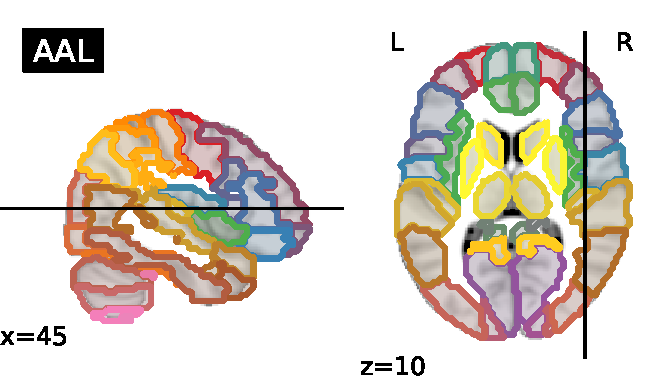
\includegraphics[width=.5\linewidth]{aal_atlas.pdf}%
\hfill%
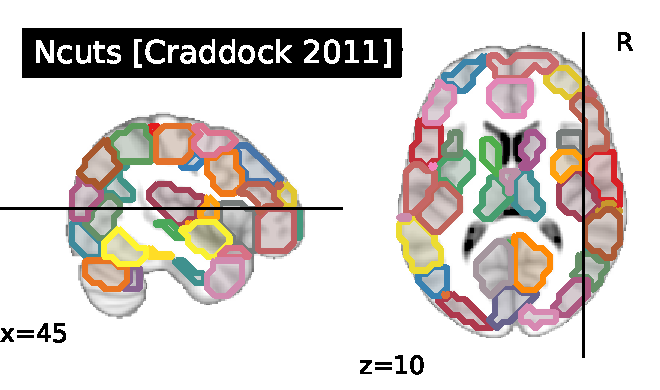
\includegraphics[width=.5\linewidth]{ncuts_atlas.pdf}%

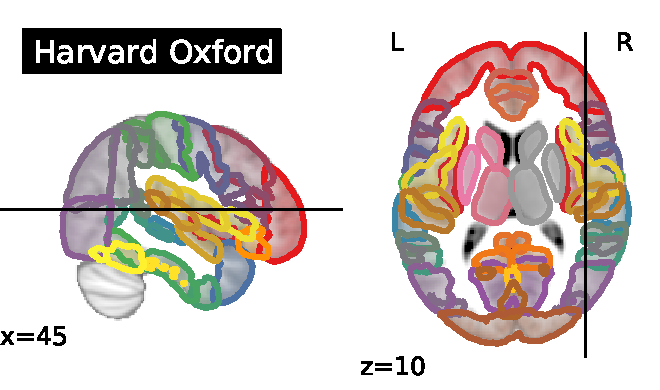
\includegraphics[width=.5\linewidth]{ho_atlas.pdf}%
\hfill%
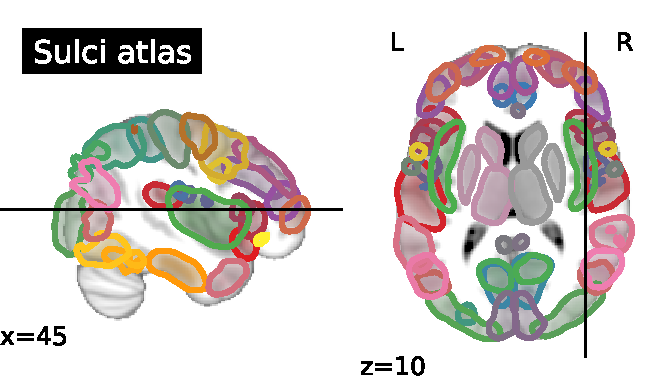
\includegraphics[width=.5\linewidth]{sulci_atlas.pdf}%

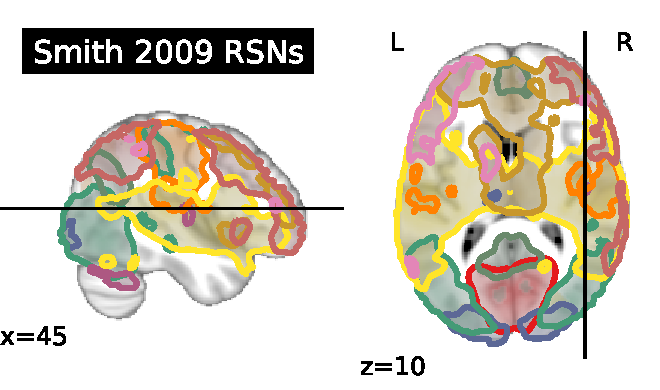
\includegraphics[width=.5\linewidth]{smith_atlas.pdf}%
\hfill%
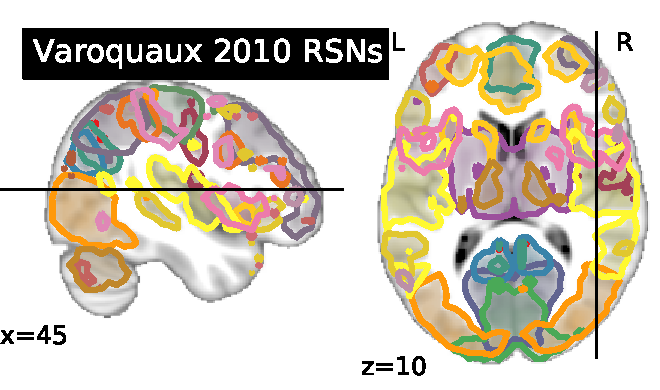
\includegraphics[width=.5\linewidth]{msdl_atlas.pdf}%

\caption{
Different regions
}
\end{figure}

%------------------------------------------------------------------------------
\subsection{Estimating connections}

% Disclaimer: focus on correlation/second order statistics?
Mutual information? Entropy correlation? MI as measure of integration (Marralec)

\paragraph{Signal extraction}

Once again separate task from rest (explain the difference between
\emph{ongoing} and \emph{evoked} activity at some point (intro?)

Task: beta time-series, and more recent stuff, \emph{e.g.} by Mumford and
Poldrack.

Rest: importance of confounds. Filtering + and detrending. Importance of
preprocessing.
Compcorr \cite{behzadi2007}
\cite{chai2011}
power, van dijk
\cite{satterthwaite2012}

FMRI signals contributing to functional connectivity
have been found to lie in frequencies below 0.1 Hz \cite{cordes2000}
XXX: but cite recent work that shows that there is info at higher
frequency.  Regressing out task??

\paragraph{Correlation and partial correlations}

Correlation, shrinkage of correlation \cite{ledoit2004,varoquaux2012},

Remark: difference between covariance and correlation matrix.

partial correlation, sparse iCov. \cite{smith2011,varoquaux2010b}. 

Give intuition on partial correlation/inverse covariance.

Remark that partial correlations consistently have no negative values.

Variety
of estimation strategies for sparse iCov, that have an impact on the
resulting network \cite{varoquaux2012}\footnote{Better estimation
algorithm is recent Honorio paper.}. Discuss setting the regularization
parameter.

%%%%%%%%%%%%%%%%%%%%%%%%%%%%%%%%%%%%%%%%%%%%%%%%%%%%%%%%%%%%%%%%%%%%%%%%%%%%%%%

\section{Comparing connections}

%------------------------------------------------------------------------------
\subsection{Mass-univariate approaches}

Boils down to a standard linear model => t-tests and co.
Stress that to have Gaussian-distributed correlations, a Fisher Z
transform is required.

Multiple comparison problem is quite an issue (scales a $p^2$) =>
permutation and max-T approach XXX: cite Ge
"resampling-based multiple testing for microarray data analysis", and
Nichols multiple comparison paper.

Family (Cameron, is that the correct name?) FWE?

%------------------------------------------------------------------------------
\subsection{Modeling between-connection dependences}

Show that correlations co-fluctuation with images, spatial correlations between correlations.

Ad-hoc model: network-based statistics \cite{zalesky2010}

Discuss the 'residual' strategy?
\cite{varoquaux2010b}

%%%%%%%%%%%%%%%%%%%%%%%%%%%%%%%%%%%%%%%%%%%%%%%%%%%%%%%%%%%%%%%%%%%%%%%%%%%%%%%

\section{Comparing Network Summary Statistics}

Small world networks, transport properties, resilient...

Warning note that correlation matrices have long-tailed degree
distribution by definition (cite recent Bullmore paper showing that).

%%%%%%%%%%%%%%%%%%%%%%%%%%%%%%%%%%%%%%%%%%%%%%%%%%%%%%%%%%%%%%%%%%%%%%%%%%%%%%%

\section{Predictive Modeling}
craddock 2009, Dosenbach 2010, lord 2011, deshpande, 

1. importance of interpretation!
2. the need for feature extraction
3. the need for feature selection
4. setting parameters.
5. different methods have different interpretations

\emph{ --- CC text from TICS paper, do not use without modification!}
Multivariate Prediction Analysis. When applied to the study of intrinsic activity, the goal of discovery
science is to identify models that relate measures of that activity (such as iFC) to phenotypic variables.
Prediction analysis provides a means for measuring how well these models generalize to independent data.
This is complementary to inferential statistics, which measure the likelihood of such relationships
arising by chance. In the prediction analysis framework, a model relating iFC to a phenotype is learned 
from a training dataset. This model is then applied to an independent test dataset to predict phenotypes.
The resultant predictions are compared to the true phenotypes to estimate how well the model generalizes
to the tese dataset. Thus, prediction analysis provides a natural framework for evaluating biomarkers [21],
performing real-time fMRI [88], and evaluating experimental tradeoffs [89]. 

Prediction analysis has been applied to functional neuroimaging data since the early 90’s [90], and more
recently to IFC data [91]. Most, if not all, analysis methods can be applied in a predictive modeling
framework but the majority of methods that have been applied to iFC are multivariate classification and
regression methods (referred to as MVPA; multivariate prediction analysis). Multivariate methods are more
sensitive to distributed patterns of iFC than their univariate counterparts. Additionally they provide a
means for evaluating the significance of an entire pattern using a single statistic, obviating the need
to correct for multiple comparisons. 

Although there are many circumstances in which high prediction accuracy is the ultimate goal of an
analysis (e.g. predicting treatment outcome), in general it is desirable that the model also be
interpretable. Identifying the iFC measures (features) that are most important to the model is
problematic and an open issue for MVPA research. Several feature selection algorithms have been proposed
to address this issue, but there is no consensus on which is best [21]. We note that feature selection
methods that rely on feature-by-feature statistical tests require correction for multiple comparisons. 

MVPA classification has already been successfully used to identify potential iFC biomarkers of Alzheimer’s
disease [92], major depression [93], schizophrenia [94], and autism [47], among others. MVPA
classification and regression techniques have also been applied to identify biomarkers of age [95,96]
and recent work has shown the utility of MVPA methods for deriving iFC models at the individual
level [97]. An in-depth overview of the statistical pattern recognition methods underlying MVPA
techniques can be found in [98].
\emph{ --- END CC text from TICS paper, do not use without modification!}


%%%%%%%%%%%%%%%%%%%%%%%%%%%%%%%%%%%%%%%%%%%%%%%%%%%%%%%%%%%%%%%%%%%%%%%%%%%%%%%

\section{Functional and effective connectivity}

Effective connectivity does not have to be causal => but a precise mathematical
definition of the relationship => BCI workshop reports

Fucntional connectivity is a statistical relationship, instead of precise mathematical
relationship

%------------------------------------------------------------------------------
\subsection{From correlations to structural equation modeling}

\cite{mcintosh1994}
\cite{marrelec2007}
\cite{marrelec2009}

%------------------------------------------------------------------------------
\subsection{Matching model complexity to data}

Diatribe: all model are wrong, but some are useful => a cat is a model of a cat

Setting the cursor between complex models based on a bio-physical
description, and simple phenomenological models such as correlation
matrices.

\cite{mcintosh2010}

Cross validation???


%%%%%%%%%%%%%%%%%%%%%%%%%%%%%%%%%%%%%%%%%%%%%%%%%%%%%%%%%%%%%%%%%%%%%%%%%%%%%%%

\section{Conclusion}

{
%\clearpage
\section*{References} \small \bibliographystyle{elsarticle-num-names}
\bibliography{biblio} }

%%%%%%%%%%%%%%%%%%%%%%%%%%%%%%%%%%%%%%%%%%%%%%%%%%%%%%%%%%%%%%%%%%%%%%%%%%%%%%%


\end{document}
